% LE HULUM -- Track 2 Software Requirements Specification
% Compile with XeLaTeX (needs the Noto Sans Ethiopic font for Amharic text):
%   xelatex le-hulum-srs.tex   (run twice for the table of contents)
% Install the STATIC Noto Sans Ethiopic files (Regular/Bold) from Google Fonts.
% On Overleaf: upload NotoSansEthiopic-Regular.ttf and NotoSansEthiopic-Bold.ttf
% next to this file, set the compiler to XeLaTeX, and change the \newfontfamily
% line below to:
%   \newfontfamily\ethfont{NotoSansEthiopic}[Path=./, Extension=.ttf,
%     UprightFont=*-Regular, BoldFont=*-Bold, Scale=0.92]

\documentclass[11pt,a4paper]{article}

\usepackage{fontspec}
\setmainfont{Latin Modern Roman}
\setsansfont{Latin Modern Sans}
\setmonofont{Latin Modern Mono}[Scale=0.95]
\newfontfamily\ethfont{Noto Sans Ethiopic}[Scale=0.92]
\newcommand{\am}[1]{{\ethfont #1}}

\usepackage[margin=2.2cm]{geometry}
\usepackage{xcolor}
\usepackage{amssymb}
\usepackage{xltabular}
\usepackage{booktabs}
\usepackage{array}
\usepackage{enumitem}
\usepackage{titlesec}
\usepackage{fancyhdr}
\usepackage{tikz}
\usetikzlibrary{positioning,arrows.meta,fit,backgrounds}
\usepackage[hidelinks]{hyperref}

\definecolor{accent}{HTML}{1F6FD1}
\definecolor{quiet}{HTML}{5F6368}
\definecolor{tint}{HTML}{F2F2F0}

\newcommand{\code}[1]{\texttt{#1}}
\newcommand{\req}[1]{\textbf{#1}}

\setlist{itemsep=2pt,topsep=4pt}
\usepackage{ragged2e}
\AtBeginDocument{\RaggedRight\sloppy}
\setlength{\emergencystretch}{3em}
\setlength{\parindent}{0pt}
\setlength{\parskip}{6pt}
\renewcommand{\arraystretch}{1.25}

\titleformat{\section}{\Large\bfseries\color{accent}}{\thesection.}{0.6em}{}
\titleformat{\subsection}{\large\bfseries}{\thesubsection}{0.6em}{}

\pagestyle{fancy}
\fancyhf{}
\lhead{\small LE HULUM (\am{ለሁሉም}) --- Track 2 SRS}
\rhead{\small Digital Bridge Accessibility Hackathon 2026}
\cfoot{\small \thepage}

\begin{document}

% ---------------------------------------------------------------- Title
\begin{titlepage}
\centering
\vspace*{3cm}
{\Huge\bfseries LE HULUM (\am{ለሁሉም})\par}
\vspace{0.4cm}
{\Large\itshape Ear to the deaf. Eye for the blind.\par}
\vspace{1.2cm}
{\Large Software Requirements Specification\par}
\vspace{0.3cm}
{\large Track 2 --- Accessible learning media\par}
\vspace{0.3cm}
{\large Digital Bridge Accessibility Hackathon 2026\par}
\vfill
{\large 14 November 2026\par}
\vspace{1cm}
\end{titlepage}

\tableofcontents
\newpage

% ---------------------------------------------------------------- 1
\section{Introduction}

LE HULUM (\am{ለሁሉም}, ``for all'') is a drop-in accessible lesson player, \code{<db-player>}, plus a server pipeline. It makes any lesson, whether a video or a text page, usable by Deaf, blind, low-vision and hard-of-hearing learners, and by learners on 3G phones, in Amharic and English.

\textbf{Main task (the gate sentence):} A Deaf, blind or hard-of-hearing learner opens a lesson (video or text) on their own low-cost Android phone on a slow connection, follows it in their preferred mode (sign, listen, read, light data) and marks it complete, with nobody helping.

\subsection{Scope}
\begin{itemize}
  \item \textbf{In scope:} the player web component, the caption and transcript pipeline, the automatic Ethiopian Sign Language (EthSL) pipeline, audio description, the offline pack, tagged HTML and PDF documents, the career gateway (job card and verifiable certificate), the REST API and open-standard outputs.
  \item \textbf{Out of scope:} sign-up and profiles (Track 1), chat assistant and live help (Track 3), payment, and any changes to Savanna's own files.
\end{itemize}

\subsection{Definitions}
\begin{xltabular}{\textwidth}{@{}l X@{}}
\toprule
\textbf{Term} & \textbf{Meaning} \\
\midrule
\endhead
EthSL & Ethiopian Sign Language \\
Cue & One caption line or sentence with a start and end time (WebVTT) \\
Gloss & Sign order written as labels, e.g.\ TODAY VARIABLE CREATE LEARN \\
Sign lexicon & Library of recorded signs, one clip per gloss \\
Translation memory & Library of verified, fully signed lesson phrases \\
Light lesson & Speech audio plus slide images, instead of video \\
Host & The site that installs the module (Savanna first) \\
Gate & Pass/fail test: co-designer completes the main task unaided; axe-core clean; WCAG 2.2 AA conformance report \\
\bottomrule
\end{xltabular}

\subsection{References}
\begin{itemize}
  \item Digital Bridge Accessibility Hackathon 2026, Track 2 brief (opening presentation, 14 Nov 2026)
  \item Team Technical Guide, version 2, 14 Nov 2026, written against \code{github.com/\allowbreak alx-africa/\allowbreak Savanna-static-pages}
  \item WCAG 2.2 AA; WebVTT; schema.org/JobPosting; Open Badges 3.0
\end{itemize}

% ---------------------------------------------------------------- 2
\section{Overall description}

The product is one script file the host loads, plus an optional server shipped in Docker Compose. Savanna has no video today; we fill that gap.

\subsection{Users and their real problems}
\begin{xltabular}{\textwidth}{@{}>{\raggedright\arraybackslash}p{2.6cm} X X@{}}
\toprule
\textbf{User} & \textbf{Real problem} & \textbf{Our answer} \\
\midrule
\endhead
Deaf learners & EthSL is the first language; written Amharic is a second. No sign on lessons; interpreters are scarce and lack technical signs & Sign-first layout, automatic EthSL from captions or text, tap-a-word sign glossary, lesson waits for the signer \\
Blind and low-vision learners & Unlabelled controls; code and slides are pixels; ``as you can see'' moments; weak Amharic phone voices & Fully labelled player, video navigable by chapter headings, ``What's on screen'' text, descriptions that pause the video, pre-recorded Amharic voice \\
Hard-of-hearing learners & Muddy audio, fast speakers, cheap speakers, one-ear hearing & Clear voice, volume boost, slow-down without pitch change, ``Say that again'', mono and balance, well-timed captions \\
Learners on slow connections & Video costs data, 3G buffers, little storage & Connection check, light lesson (audio + slides), resumable offline packs, single-file sharing, offline progress \\
Content providers and platforms & No time or staff to make lessons accessible & Studio: AI drafts, quick human review, automatic outputs; one script tag to install \\
\bottomrule
\end{xltabular}

\subsection{Constraints from the Technical Guide}
\begin{itemize}
  \item \req{C-01} It is a module, not an app: one script, \code{module/db-player.js}, configured only by attributes.
  \item \req{C-02} It mounts in \code{savanna/\allowbreak pages/\allowbreak concept-with-navigation.html}, inside \code{\#curriculum\_\allowbreak navigation\_\allowbreak content} \code{.savanna-styles}, under the banner image.
  \item \req{C-03} It must also work and look right on \code{demo/blank.html}, with no Bootstrap and no Savanna CSS.
  \item \req{C-04} CSS lives in a shadow root. Host look comes from \code{var(--bs-primary)}, \code{var(--bs-body-\allowbreak font-family)}, \code{var(--bs-body-color)}, with fallbacks.
  \item \req{C-05} No edits to Savanna's files, no global variables, no changes to \code{window} or \code{document.\allowbreak body}.
  \item \req{C-06} First load under 500 KB (our target: under 60 KB of player code).
  \item \req{C-07} All text in \code{i18n/en.json} and \code{i18n/am.json}; no sentence in code. A new language is one new JSON file.
  \item \req{C-08} Talk to the host only through events (\code{db-player:*}, \code{bubbles} + \code{composed}).
  \item \req{C-09} Microphone, camera and service workers need HTTPS: test on phones through a \code{cloudflared} or \code{ngrok} tunnel.
  \item \req{C-10} The module stays useful with no AI at all. Every AI step sits behind a server-side switch.
  \item \req{C-11} Test content only: our own 1--2 minute lesson clip, test jobs in a JSON file. No real names, phones or documents.
\end{itemize}

\subsection{Assumptions}
\begin{itemize}
  \item Learners mostly use Chrome on low-cost Android phones.
  \item On-site EthSL interpreters and a Deaf co-designer help record the starter sign lexicon and phrase library on day 1.
  \item ALX names the open licence at kick-off; every library we use is permissive and listed.
\end{itemize}

% ---------------------------------------------------------------- 3
\section{Functional requirements: player core and learner profile}

The player is a custom web component on the native \code{<video>} element. It follows Able Player's tested patterns but runs our own code, so that sign sync, description pauses and the light lesson share one clock.

\subsection{Embedding}
\begin{itemize}
  \item \req{FR-CORE-01} The host installs it with one tag:
\begin{verbatim}
<db-player src="lesson.mp4"
           captions="lesson.en.vtt,lesson.am.vtt"
           sign="lesson.ethsl.mp4" describe="lesson.ad.mp3"
           lang="am" api="https://.../api/v1"
           lesson-id="python-01"></db-player>
\end{verbatim}
  \item \req{FR-CORE-02} If \code{api} and \code{lesson-id} are set, the player loads all tracks (captions, sign track, descriptions, chapters, slides, screen text) from \code{GET /api/v1/lessons/\{id\}}. Without them it uses the attributes alone.
  \item \req{FR-CORE-03} It emits \code{db-player:progress \{seconds, percent\}}, \code{db-player:complete \{\}} and \code{db-player:prefs \{captionSize, captionColor, signPosition, ...\}}.
  \item \req{FR-CORE-04} No autoplay. \code{preload="none"} and a small poster image until the learner chooses a mode.
\end{itemize}

\subsection{Controls}
\begin{itemize}
  \item \req{FR-CORE-05} Every control is a real \code{<button>} or \code{<input>} with a name: Play/Pause, Back 10 seconds, Forward 10 seconds, Speed, Captions, Sign language, Audio description, Transcript, What's on screen, Settings, Full screen, Keyboard help.
  \item \req{FR-CORE-06} The Play button's text changes to ``Pause''. The seek slider speaks in words via \code{aria-valuetext} (``1 minute 10 seconds of 5 minutes'').
  \item \req{FR-CORE-07} Settings use plain show/hide panels and \code{<dialog>} with \code{showModal()}, never complex ARIA menus.
  \item \req{FR-CORE-08} Every state change is announced in a polite \code{aria-live} region (``Captions on'', ``Jumped to Chapter 3'').
  \item \req{FR-CORE-09} Full screen keeps focus inside the player, and controls never vanish beyond keyboard reach.
\end{itemize}

\subsection{Keyboard}
\begin{itemize}
  \item \req{FR-CORE-10} Shortcuts work only while focus is inside the player, are ignored in text fields, and can be turned off (WCAG 2.1.4).
  \item \req{FR-CORE-11} Map: Space and K play/pause; Left/Right arrows and J/L seek 10 s; C captions; S sign; D description; T transcript; W what's on screen; R say that again; ? keyboard help.
  \item \req{FR-CORE-12} Every shortcut also exists as a visible, labelled button, for TalkBack users.
  \item \req{FR-CORE-13} Optional sound cues (earcons) for play, pause and ``description coming'', generated with Web Audio (no files).
\end{itemize}

\subsection{Learner profile: ``How do you want to learn?''}
\begin{itemize}
  \item \req{FR-PROF-01} On first open, one screen offers four large choices, any combination: Sign, Listen, Read, Save data.
  \item \req{FR-PROF-02} The choice sets defaults: Sign $\rightarrow$ sign-first layout; Listen $\rightarrow$ Clear voice, captions below the video, 150\% boost; Read $\rightarrow$ transcript open; Save data $\rightarrow$ light lesson.
  \item \req{FR-PROF-03} No medical question, no proof. Choices and all settings are stored only on the device (\code{localStorage}) and can be changed any time.
  \item \req{FR-PROF-04} Settings are never sent to the server or to an employer.
\end{itemize}

\subsection{Captions and transcript (shared by all users)}
\begin{itemize}
  \item \req{FR-CAP-01} Captions come from WebVTT, one file per language. The player reads cues itself (\code{track.mode = "hidden"} + \code{cuechange}) and draws them in its own element. Never captions burned into the picture.
  \item \req{FR-CAP-02} Learner settings: size 100--300\%, text colour, background colour and opacity, position (bottom over video, top over video, below the video). Saved and re-applied.
  \item \req{FR-CAP-03} Amharic uses Noto Sans Ethiopic (bundled), line height about 1.7, no all-caps or letter spacing, and \code{lang="am"} on Amharic text.
  \item \req{FR-CAP-04} Speaker names (\code{<v Teacher>}) shown as name plus colour, never colour alone; sound events like \code{[music]} in italics. Every meaningful sound has a caption (sound-off check).
  \item \req{FR-TRN-01} The transcript is built from the same VTT. Each line is a button that seeks there; the current line is highlighted and marked \code{aria-current}.
  \item \req{FR-TRN-02} The transcript never auto-scrolls while focus is inside it.
  \item \req{FR-TRN-03} The transcript downloads as plain text.
\end{itemize}

\subsection{Two input types: video or text}
A lesson can be a video or a text page (like Savanna's own concept page). Both become the same thing inside LE HULUM: a list of timed sentences (cues), so every feature in this document works for both.
\begin{itemize}
  \item \req{FR-IN-01} Accepted input: video (MP4) or text (HTML or Markdown, including the host's existing lesson page).
  \item \req{FR-IN-02 Text mode on the host page.} This tag attaches to an existing lesson:
\begin{verbatim}
<db-player for="#curriculum_navigation_content .savanna-styles"
           lang="am"></db-player>
\end{verbatim}
It adds a toolbar (Sign, Listen, Translate, Download) above the text and never rewrites the host's markup.
  \item \req{FR-IN-03 Sentence cues.} The server splits the text by headings into sections and by sentence into cues. Headings become chapters; code blocks and lists stay intact.
  \item \req{FR-IN-04 Sign for text.} Each sentence goes through the EthSL pipeline (section~\ref{sec:ethsl}). The sign window plays sentence by sentence while the current sentence is highlighted in the text, so a Deaf learner sees the words and the sign together.
  \item \req{FR-IN-05 Listen for text.} Each sentence gets pre-rendered narration (Amharic or English TTS). Sentence timings come from the audio durations, so play, pause, seek, speed, Clear voice and Say that again work exactly as for video.
  \item \req{FR-IN-06 Read-along without touching the host.} The current sentence is highlighted with the CSS Custom Highlight API (\code{CSS.highlights}), which marks text ranges without changing the host's elements. Fallback: a read-along copy inside our shadow root.
  \item \req{FR-IN-07 Translate.} English text lessons get an Amharic version (MADLAD-400 draft, human review), switchable from the toolbar, with \code{lang} set on each version.
  \item \req{FR-IN-08 Images in text.} Every image needs a real description: the author's own, or an AI draft reviewed in the Studio. Never the file name (a defect the starter has).
  \item \req{FR-IN-09 Offline for text.} The Text pack is the lesson itself (about 50 KB); the Light pack adds narration audio; sign clips are optional.
  \item \req{FR-IN-10 Same events and API.} Text lessons emit the same \code{db-player:*} events and use the same \code{/api/v1/lessons/\{id\}} endpoints, with \code{type: video | text} in the metadata.
\end{itemize}

% ---------------------------------------------------------------- 4
\section{Functional requirements: Deaf learners and automatic EthSL}

Sign language is the main access route for Deaf learners, so every lesson gets an EthSL track automatically, and the player gives that track the space and timing it needs.

\subsection{Sign window and layout}
\begin{itemize}
  \item \req{FR-DEAF-01 Sign-first layout.} In Sign mode the signer is large and the lesson video small. The L key or a Swap button toggles back.
  \item \req{FR-DEAF-02 Movable, resizable window.} In lesson-first mode the sign window floats. It can be moved by drag (mouse and touch), by arrow keys (5\% steps) and by \textbf{position buttons}: top left, top right, bottom left, bottom right. Larger/Smaller buttons and +/$-$ resize it with the aspect ratio locked. Dragging is never the only way (WCAG 2.5.7).
  \item \req{FR-DEAF-03} Opacity choice 100\% / 80\% / 60\%. Minimum size keeps hands and face readable.
  \item \req{FR-DEAF-04} Position, size, opacity and layout are saved on the device and announced when changed.
\end{itemize}

\subsection{Sign timing}
\begin{itemize}
  \item \req{FR-DEAF-05 Two sign sources.} (a) A continuous interpreted video (\code{sign} attribute): on play, pause, seek and ratechange, copy \code{currentTime} and \code{playbackRate}, and correct drift once a second. (b) A per-cue sign track (\code{sign.json}), one clip per caption line or sentence, as produced by the pipeline below.
  \item \req{FR-DEAF-06 Lag-aware sync.} With a per-cue track, when the lesson reaches the end of a line before its sign clip ends, the lesson pauses and resumes when the clip finishes. A visible ``Waiting for signer...'' badge shows the pause is deliberate. Learner pauses and automatic pauses are tracked separately. A ``Wait for signer'' switch, on by default.
  \item \req{FR-DEAF-07 Slow signer.} The sign video plays at 1 / 0.85 / 0.75 speed independently; lag-aware sync keeps the lesson in step.
  \item \req{FR-DEAF-08 No sign yet.} If a lesson has no sign track, the player says so in words, shows captions with tappable glossary signs, and offers ``Request sign for this lesson''.
\end{itemize}

\subsection{Tap-a-word sign glossary}
\begin{itemize}
  \item \req{FR-DEAF-09} Technical terms in the transcript and captions are buttons (\code{aria-label=} \code{"variable,} \code{show sign"}). Tapping pauses the lesson and opens a \code{<dialog>} with the looping sign clip and the word in English and Amharic. Focus returns to the word on close.
  \item \req{FR-DEAF-10} A ``Signs in this lesson'' list under the player lets learners preview all terms first.
  \item \req{FR-DEAF-11} Terms are matched by longest match, case-insensitive, including listed Amharic word forms.
\end{itemize}

\subsection{Automatic EthSL pipeline (server)}\label{sec:ethsl}
The system translates every Amharic caption line or text sentence into an EthSL video with no interpreter per lesson. Humans record each sign or phrase \textbf{once}; the system builds every lesson from those recordings. The design follows the open University of Zurich text $\rightarrow$ gloss $\rightarrow$ pose $\rightarrow$ video pipeline, two AAU theses on Amharic-to-EthSL, and Signapse's phrase-library approach.

\begin{center}
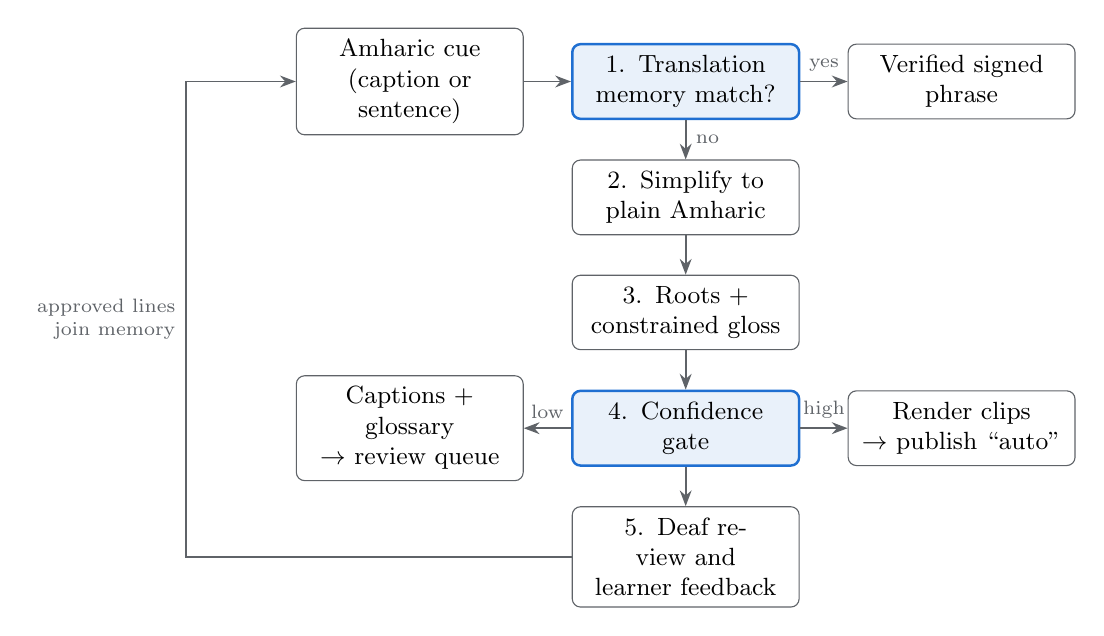
\begin{tikzpicture}[
  node distance=5mm and 6mm,
  stp/.style={draw=quiet, rounded corners=3pt, align=center, font=\small, minimum height=8mm, inner sep=4pt, text width=2.6cm},
  key/.style={stp, draw=accent, fill=accent!10, line width=0.9pt},
  arr/.style={-{Stealth[length=2mm]}, quiet, line width=0.7pt}]
\node[stp] (in) {Amharic cue\\(caption or sentence)};
\node[key, right=of in] (mem) {1. Translation\\memory match?};
\node[stp, right=of mem] (pub1) {Verified signed\\phrase};
\node[stp, below=of mem] (simp) {2. Simplify to\\plain Amharic};
\node[stp, below=of simp] (root) {3. Roots +\\constrained gloss};
\node[key, below=of root] (gate) {4. Confidence\\gate};
\node[stp, right=of gate] (pub2) {Render clips\\$\rightarrow$ publish ``auto''};
\node[stp, left=of gate] (rev) {Captions + glossary\\$\rightarrow$ review queue};
\node[stp, below=of gate] (fb) {5. Deaf review and\\learner feedback};
\draw[arr] (in) -- (mem);
\draw[arr] (mem) -- node[above, font=\scriptsize] {yes} (pub1);
\draw[arr] (mem) -- node[right, font=\scriptsize] {no} (simp);
\draw[arr] (simp) -- (root);
\draw[arr] (root) -- (gate);
\draw[arr] (gate) -- node[above, font=\scriptsize] {high} (pub2);
\draw[arr] (gate) -- node[above, font=\scriptsize] {low} (rev);
\draw[arr] (gate) -- (fb);
\draw[arr] (fb.west) -| node[pos=0.75, left, font=\scriptsize, align=right] {approved lines\\join memory} ([xshift=-14mm]in.west) |- (in.west);
\end{tikzpicture}
\end{center}

\begin{itemize}
  \item \req{FR-SL-01 Input.} Corrected Amharic caption cues from a video, or sentences from a text lesson. English input is translated to Amharic first (MADLAD-400).
  \item \req{FR-SL-02 Layer 1, translation memory.} Each cue is matched against verified, fully signed phrases using meaning-based (embedding) similarity. A match above threshold uses the verified human-signed phrase directly.
  \item \req{FR-SL-03 Layer 2, simplify.} Unmatched lines are rewritten into plain Amharic: short sentences, one idea each, no idioms.
  \item \req{FR-SL-04 Layer 3, roots.} Words are reduced to roots with an Amharic morphological analyser (HornMorpho).
  \item \req{FR-SL-05 Layer 3, constrained glossing.} An AI produces the gloss from the closest verified example pairs (retrieved, about 30), may only output glosses that exist in the lexicon or fingerspelling, and is checked by a rule engine (time words first, negation, question position). Rules are written with the interpreters and the Deaf co-designer, not invented.
  \item \req{FR-SL-06 Layer 4, confidence gate.} Each line gets a score from: memory match, share of words with a real sign (vs fingerspelled), agreement of 3 independent gloss attempts, and rule pass. High confidence $\rightarrow$ published as ``Automatic sign (beta)''. Low $\rightarrow$ captions plus glossary signs, and the line goes to the review queue.
  \item \req{FR-SL-07 Rendering.} Prefer whole phrases, then word clips, then fingerspelling. Clips are trimmed of rest holds, joined with 0.10--0.15 s crossfades (ffmpeg), same signer, background, lighting and framing. Real video keeps the face, which carries EthSL grammar. Pose-based avatar (MediaPipe keypoints, a few KB per sentence) is a stretch goal.
  \item \req{FR-SL-08 Fingerspelling fallback.} Any word with no sign is fingerspelled from the recorded Ethiopian manual alphabet, so every word always renders.
  \item \req{FR-SL-09 Layer 5, Deaf review.} A reviewer sees line, gloss and video and taps Approve / Fix order / Missing sign. Approved lines join the translation memory automatically.
  \item \req{FR-SL-10 Learner feedback.} Thumbs up / thumbs down on each auto-signed line; flagged lines go to review.
  \item \req{FR-SL-11 Coverage shown.} The player and Studio show ``X\% of lines signed, Y\% of words fingerspelled''.
  \item \req{FR-SL-12 Honest labelling.} Machine output is always labelled. The AI layer is pluggable (cloud, local open model, or rules only) and runs once per lesson, not live.
\end{itemize}

\subsection{Lexicon and memory recording}
\begin{itemize}
  \item \req{FR-SL-13} A phone recording page records lexicon signs and phrases one at a time (front camera, \code{getUserMedia} + \code{MediaRecorder}), with retake and next.
  \item \req{FR-SL-14} Uploads are compressed for 3G: \code{scale=-2:288} (lexicon) or \code{-2:360}, \code{fps=20}, no audio, H.264 \code{-preset veryfast -crf 30}.
  \item \req{FR-SL-15} Lexicon entry format: \code{\{gloss, am:[forms], en:[forms], clip, pose?\}}. Phrase entry: \code{\{text\_am, gloss, clip, verified\_by, date\}}.
  \item \req{FR-SL-16} Day-1 recording target: 20--30 common lesson phrases, about 100 word signs (each signed inside a short sentence), the fingerspelling alphabet, and 30 interpreter-written glosses (20 examples, 10 held out for the test).
\end{itemize}

\subsection{Sound shown as text}
\begin{itemize}
  \item \req{FR-DEAF-12} Captions show speaker name and colour and sound events, entered in the caption editor.
\end{itemize}

% ---------------------------------------------------------------- 5
\section{Functional requirements: blind and low-vision learners}

A blind learner can operate everything by screen reader, skim the lesson like a document, read the exact code on screen, and hear what the teacher points at.

\subsection{Navigate the video like a document}
\begin{itemize}
  \item \req{FR-BLV-01 Automatic chapters.} The server detects scene changes (\code{ffmpeg select='gt(scene,0.3)'}), merges changes less than 20 s apart, and titles each chapter from the slide's title text (OCR) or a 3--6 word AI summary. A person can rename them. Saved as \code{chapters.vtt}.
  \item \req{FR-BLV-02} The transcript renders as a document: a chapter list in \code{<nav>}, then one \code{<section>} per chapter with a real \code{<h3>}, and each caption line as a button that plays from that point. NVDA users press H; TalkBack users swipe by heading.
\end{itemize}

\subsection{What's on screen}
\begin{itemize}
  \item \req{FR-BLV-03 Server.} One frame at every scene change and every 5 s; Tesseract OCR (\code{-l eng+amh --psm 6}, line structure kept); duplicates dropped; optional AI fix of OCR errors in code, marked for checking. Saved as \code{screen.json} \code{[\{start, end, kind: code|slide, text\}]}. Source video for OCR is 720p or higher.
  \item \req{FR-BLV-04 Player.} W or the button pauses the lesson, opens a panel, and moves focus to its heading ``On screen at 1:10''. Code is in \code{<pre><code>}, readable line by line and character by character. A Copy code button. Escape closes and returns focus.
\end{itemize}

\subsection{Audio description}
\begin{itemize}
  \item \req{FR-BLV-05 Find the moments.} The server flags (a) pointing phrases in the transcript (``as you can see'', ``look at'', ``like this'', \am{እዚህ}, \am{ይህን}, \am{እንደምታዩት}, \am{ተመልከቱ}) and (b) visual changes during 3 s or more of silence.
  \item \req{FR-BLV-06 Drafts.} Code and slide moments are drafted from OCR; other visuals by a pluggable vision AI. A person edits only the flagged moments in the Studio.
  \item \req{FR-BLV-07 Format.} Descriptions are \code{descriptions.vtt} (Amharic and English), each cue pointing to its pre-made audio file. A pre-mixed \code{describe} audio file is also accepted.
  \item \req{FR-BLV-08 Extended description.} On a description cue the video pauses, a short tone plays, the description plays, then the video resumes. It never talks over the teacher.
  \item \req{FR-BLV-09 Two modes, learner's choice.} Voice (our pre-recorded audio) or Screen reader (text sent to the live region, read by the learner's own screen reader at their own speed). Fallback: \code{speechSynthesis} when neither audio nor a screen reader is available.
  \item \req{FR-BLV-10} Separate sliders for lesson volume and description volume. Optional ducking to 30\% for short descriptions.
\end{itemize}

\subsection{Real Amharic voice}
\begin{itemize}
  \item \req{FR-BLV-11} A server job turns every description and job-card summary into speech with an open Amharic TTS model (swappable through one function), saved as Opus 24 kbps (\code{ad/<cue>.am.opus}). English uses an open English voice. The phone never needs an Amharic voice installed.
\end{itemize}

\subsection{Low vision}
\begin{itemize}
  \item \req{FR-BLV-12} High-contrast theme (yellow on black) and automatic use of \code{prefers-contrast: more}.
  \item \req{FR-BLV-13} Reflow at 200\% and 400\% zoom and at 320 px width: controls wrap, no sideways scrolling, no fixed heights. Sizes in rem.
  \item \req{FR-BLV-14} Targets at least 44 $\times$ 44 px; \code{:focus-visible} outline 3 px; nothing sticky covers the focused element.
  \item \req{FR-BLV-15} Contrast at least 4.5:1 for text and 3:1 for controls. No text inside images. \code{prefers-reduced-motion} respected.
\end{itemize}

% ---------------------------------------------------------------- 6
\section{Functional requirements: hard-of-hearing learners}

All hearing features run on the phone through one Web Audio chain, with no server and no extra data.

\subsection{Audio chain}
\begin{itemize}
  \item \req{FR-HOH-01} Chain built once, on the first Play press: source $\rightarrow$ high-pass 100 Hz $\rightarrow$ peaking 2.5 kHz $\rightarrow$ peaking 4 kHz $\rightarrow$ compressor $\rightarrow$ gain (boost) $\rightarrow$ mono/balance $\rightarrow$ output. The same chain attaches to the \code{<audio>} element in light-lesson and text-narration mode.
  \item \req{FR-HOH-02} The video carries \code{crossorigin="anonymous"} and the server sends CORS headers; otherwise Web Audio outputs silence.
\end{itemize}

\subsection{Features}
\begin{itemize}
  \item \req{FR-HOH-03 Clear voice.} Off / Clear / Extra clear: 0 / +6 / +9 dB at 2.5 kHz, 0 / +3 / +6 dB at 4 kHz, compressor ratio 1 / 4 / 6.
  \item \req{FR-HOH-04 Volume boost.} 100\% / 150\% / 200\%, with the compressor preventing distortion.
  \item \req{FR-HOH-05 Slow down.} 1 / 0.85 / 0.75 speed with \code{preservesPitch = true}. Sign sync follows automatically.
  \item \req{FR-HOH-06 Say that again.} R or a button replays the last caption line from 0.2 s before its start, with the caption shown larger. A second press within 2 s goes one more line back. Long-press or Shift+R repeats at 0.75 speed.
  \item \req{FR-HOH-07 Mono and balance.} A mono switch mixes both channels into both ears; a balance slider pans towards the better ear.
\end{itemize}

\subsection{Captions for people who also listen}
\begin{itemize}
  \item \req{FR-HOH-08 Timing.} English: faster-whisper with word timestamps. Amharic: forced alignment of the corrected transcript (torchaudio aligner with a CTC model such as Omnilingual ASR).
  \item \req{FR-HOH-09 Line rules.} Break at natural pauses; at most 2 lines of about 42 characters; each cue on screen 1--7 s.
  \item \req{FR-HOH-10 Default position} below the video in Listen mode, so captions never cover slides or code.
  \item \req{FR-HOH-11 Confidence.} Words with recognition probability under 0.5 are tagged \code{<c.low>} in the VTT and shown with a dotted underline (switchable). Reviewing a line removes the tags. The player shows ``Captions: X\% checked by a person''.
\end{itemize}

\subsection{Hearing settings panel}
\begin{itemize}
  \item \req{FR-HOH-12} One labelled panel: Clear voice, Volume boost, Speed, Mono, Balance, caption size/colour/background/position, Show uncertain words.
\end{itemize}

% ---------------------------------------------------------------- 7
\section{Functional requirements: slow connection, offline pack and documents}

The server prepares several small versions of every lesson; the phone downloads only the smallest one that works and shows the size before any download.

\subsection{Renditions (server, one job per upload)}
\begin{xltabular}{\textwidth}{@{}l X l@{}}
\toprule
\textbf{Version} & \textbf{How} & \textbf{Size, 5-min lesson} \\
\midrule
\endhead
Video 720p & source & about 40 MB \\
Video 360p & \code{-vf scale=-2:360 -b:v 350k} & about 15 MB \\
Speech audio & \code{-ac 1 -c:a libopus -b:a 24k -application voip} & about 0.9 MB \\
Slides & one WebP per scene change, \code{scale=854:-2}, quality 60 & about 0.5 MB \\
Text & captions, transcript, chapters, screen text, descriptions & about 50 KB \\
Sign video & cropped to signer, \code{scale=-2:288}, \code{fps=20}, no audio & about 3--5 MB \\
\bottomrule
\end{xltabular}
\begin{itemize}
  \item \req{FR-NET-01} All versions are listed with exact byte sizes in \code{manifest.json}.
\end{itemize}

\subsection{Choosing what to play}
\begin{itemize}
  \item \req{FR-NET-02} Before playing, the player checks \code{navigator.connection} (\code{saveData}, \code{effectiveType}) or times a 20 KB probe download.
  \item \req{FR-NET-03} It offers a choice with real sizes (Light lesson / Video / Text only), the right one pre-selected, remembered for next time.
\end{itemize}

\subsection{Light lesson}
\begin{itemize}
  \item \req{FR-NET-04} Speech audio is the clock; the slide image changes at each scene time, with the next slide preloaded. Each slide has \code{alt} text from OCR and descriptions.
  \item \req{FR-NET-05} All other features work in light mode: captions, transcript, glossary, sign track, say that again, Clear voice, descriptions, what's on screen.
  \item \req{FR-NET-06} Sign video in light mode streams only the clip for the current line.
\end{itemize}

\subsection{Offline pack}
\begin{itemize}
  \item \req{FR-NET-07} ``Download for offline'' offers three packs with sizes shown before the tap: Text (about 50 KB), Light (about 1.5 MB per 5 min), Full (adds video and sign).
  \item \req{FR-NET-08} A service worker with Cache Storage holds the pack; \code{navigator.storage.persist()} is requested.
  \item \req{FR-NET-09} Large files download in 256 KB HTTP Range chunks saved to IndexedDB, so an interrupted download resumes where it stopped. Background Fetch is used where available.
  \item \req{FR-NET-10} ``My downloads'' lists lessons, storage used, and a delete button.
  \item \req{FR-NET-11} The lesson works fully in aeroplane mode: playback, captions, transcript, descriptions, glossary.
\end{itemize}

\subsection{Share as one file}
\begin{itemize}
  \item \req{FR-NET-12} \code{GET /api/v1/lessons/\{id\}/offline-pack} returns one self-contained \code{lesson.html} with a tiny player, text, slides and audio embedded (about 2 MB for a light lesson). It opens in any phone browser with no internet.
  \item \req{FR-NET-13} A Share button uses \code{navigator.share(\{files\})} so the learner sends it through Telegram, Bluetooth or any app. Fallback if Android blocks local HTML: share a link to the in-app download.
\end{itemize}

\subsection{Tagged documents}
\begin{itemize}
  \item \req{FR-DOC-01} The lesson as clean HTML: headings in order, \code{lang} attributes, code blocks, and a real description for every image (never the file name). The same HTML is the Text pack.
  \item \req{FR-DOC-02} Tagged PDF/UA from that HTML with WeasyPrint (\code{--pdf-variant pdf/ua-1}), checked with a PDF accessibility validator; result stated honestly.
  \item \req{FR-DOC-03 (extra)} Braille export \code{.brf} from the transcript with liblouis (Ethiopic and English tables).
  \item \req{FR-DOC-04 (extra)} Recorded live-session viewer: the chat log becomes a timed track shown in the transcript panel. Stretch only.
\end{itemize}

\subsection{Offline progress}
\begin{itemize}
  \item \req{FR-NET-14} Progress events (chapter done, complete) are queued in IndexedDB with a unique id and sent on the \code{online} event or Background Sync. The server ignores duplicates.
  \item \req{FR-NET-15} The learner sees ``Saved on this phone. It will send when you are online.''
\end{itemize}

\subsection{Performance budget}
\begin{itemize}
  \item \req{FR-NET-16} Player code under 60 KB compressed; heavy features load only when turned on. Usable within 3 s on Chrome ``Slow 3G'' with 4$\times$ CPU slowdown. Measured time and size are written in the README.
\end{itemize}

% ---------------------------------------------------------------- 8
\section{Functional requirements: career gateway and Studio}

The career gateway reuses the player's audio, sign and offline parts on a demo jobs page; the Studio is where lessons are made accessible with AI drafts and short human reviews.

\subsection{Accessible job card}
\begin{itemize}
  \item \req{FR-JOB-01} A \code{<db-job-card>} component on \code{savanna/pages/jobs.html}, fed by test jobs in \code{demo/data/jobs.json}.
  \item \req{FR-JOB-02} ``Listen to summary'' plays a pre-rendered Amharic or English audio summary (same TTS job as descriptions); \code{speechSynthesis} fallback.
  \item \req{FR-JOB-03} Optional signed summary clip (from the EthSL pipeline) and a Text-only light view.
  \item \req{FR-JOB-04} Works at 200\% zoom and 320 px width with no sideways scrolling; real headings, buttons and links.
  \item \req{FR-JOB-05} Dates in both calendars via the browser's built-in \code{Intl.\allowbreak DateTimeFormat(} \code{'am-ET-u-ca-ethiopic', ...)} next to the Gregorian date.
  \item \req{FR-JOB-06} Each job is also embedded as schema.org \code{JobPosting} JSON-LD.
  \item \req{FR-JOB-07} The job card never shows or sends the learner's access settings.
\end{itemize}

\subsection{Verifiable certificate}
\begin{itemize}
  \item \req{FR-CERT-01} On \code{db-player:complete} for a course, the server issues an Open Badges 3.0 credential: signed JSON with issuer, learner, achievement and date.
  \item \req{FR-CERT-02} A certificate page shows the achievement, a verify link and a QR code; dates in both calendars.
  \item \req{FR-CERT-03} The verify page checks the signature and shows ``valid'' or ``not valid'' in words. It shows no disability or access information.
  \item \req{FR-CERT-04} Signing keys stay on the server and come from \code{.env}; a test key is used for the demo.
\end{itemize}

\subsection{Studio (provider side)}
\begin{itemize}
  \item \req{FR-STU-01 Upload.} A provider uploads a video or a text lesson (HTML or Markdown); the pipeline makes renditions, captions (open ASR draft), chapters, screen text, flagged description moments, Amharic translation, EthSL track, and audio.
  \item \req{FR-STU-02 Caption editor.} One line per row: text, start, end, speaker, sound events. Low-confidence words highlighted. Export to VTT. Accessible by keyboard and screen reader.
  \item \req{FR-STU-03 Description editor.} Only the flagged moments, each with its draft; save regenerates audio.
  \item \req{FR-STU-04 Sign review queue.} Line, gloss and video side by side; Approve / Fix order / Missing sign.
  \item \req{FR-STU-05 Recording page.} Records lexicon signs, phrases and fingerspelling (FR-SL-13).
  \item \req{FR-STU-06 Lesson score.} Captions checked \%, sign coverage \%, descriptions done, offline pack ready.
  \item \req{FR-STU-07 Measured quality.} The Studio reports caption accuracy on a checked sample and EthSL understandability from Deaf ratings, for the README.
\end{itemize}

% ---------------------------------------------------------------- 9
\section{Integration: script tag, REST API, open standards}

We ship Level 1 and Level 2 fully, and Level 3 through JobPosting and Open Badges 3.0; LTI 1.3 is documented only, as the guide advises.

\subsection{Level 1: script tag}
\begin{itemize}
  \item \req{INT-01} \code{<script src=".../module/db-player.js" defer></script>} then \code{<db-player ...>}; same for \code{<db-job-card>}.
  \item \req{INT-02} Proven twice: inside \code{savanna/\allowbreak pages/\allowbreak concept-with-navigation.html} and on \code{demo/blank.html} with no Bootstrap.
  \item \req{INT-03} Attributes: \code{src}, \code{for} (text mode), \code{captions}, \code{sign}, \code{describe}, \code{lang}, \code{api}, \code{lesson-id}, \code{theme}.
  \item \req{INT-04} Events: \code{db-player:progress \{seconds, percent\}}, \code{db-player:complete \{\}}, \code{db-player:prefs \{...\}}, \code{db-player:mode \{mode\}}.
\end{itemize}

\subsection{Level 2: REST API (\code{/api/v1}, FastAPI)}
{\footnotesize
\begin{xltabular}{\textwidth}{@{}l >{\raggedright\arraybackslash}p{6.4cm} X@{}}
\toprule
\textbf{Method} & \textbf{Path} & \textbf{Purpose} \\
\midrule
\endhead
GET & \code{/api/v1/lessons/\{id\}} & Metadata and list of all tracks (manifest) \\
POST & \code{/api/v1/lessons} & Upload a video or a text lesson; starts the pipeline, returns 201 \code{\{id\}} \\
GET & \code{/api/v1/lessons/\{id\}/transcript?lang=am} & Transcript text \\
POST & \code{/api/v1/lessons/\{id\}/captions} & Upload or correct a caption file \\
GET & \code{/api/v1/lessons/\{id\}/chapters} & \code{chapters.vtt} \\
GET & \code{/api/v1/lessons/\{id\}/screen} & \code{screen.json} \\
GET & \code{/api/v1/lessons/\{id\}/descriptions?lang=am} & \code{descriptions.vtt} \\
GET & \code{/api/v1/lessons/\{id\}/sign} & \code{sign.json} \\
GET & \code{/api/v1/lessons/\{id\}/offline-pack?level=...} & One downloadable file (text, light or full) \\
GET & \code{/api/v1/lessons/\{id\}/document.pdf} & Tagged PDF/UA \\
GET & \code{/api/v1/lessons/\{id\}/document.brf} & Braille (extra) \\
GET, POST & \code{/api/v1/glossary} & Sign glossary terms \\
GET, POST & \code{/api/v1/lexicon} & Sign lexicon entries and clips \\
GET, POST & \code{/api/v1/phrases} & Translation memory \\
POST & \code{/api/v1/sign/translate} & Amharic text to \code{\{gloss, confidence, clip\}} \\
POST & \code{/api/v1/sign/review/\{cue\}} & Approve / fix / missing sign \\
POST & \code{/api/v1/progress} & Batched progress events (idempotent) \\
POST & \code{/api/v1/certificates} & Issue an Open Badges 3.0 credential \\
GET & \code{/api/v1/certificates/\{id\}/verify} & valid / not valid \\
GET & \code{/api/v1/jobs} & Test jobs with JobPosting fields \\
POST & \code{/api/v1/webhooks} & Register a host address for \code{lesson.completed} \\
\bottomrule
\end{xltabular}
}
\begin{itemize}
  \item \req{INT-05} JSON, standard verbs and codes (201, 400 with a message in words, 404). \code{openapi.yaml} at the repo root, Swagger UI at \code{/docs}, one curl example per call in the README.
  \item \req{INT-06} One webhook: the server posts \code{lesson.completed} to the host's registered address.
\end{itemize}

\subsection{Level 3: open standards}
\begin{itemize}
  \item \req{INT-07} schema.org \code{JobPosting} JSON-LD on every job.
  \item \req{INT-08} Open Badges 3.0 certificates with signature verification.
  \item \req{INT-09} LTI 1.3: a clear README section on how the player would launch inside Moodle or Canvas. Built only if time remains after everything else passes.
\end{itemize}

\subsection{Data formats (open, documented)}
\begin{itemize}
  \item \req{INT-10} Standard WebVTT for captions (\code{<v>} speakers, \code{<c.low>} confidence), chapters and descriptions.
  \item \req{INT-11} \code{sign.json}: \code{\{lesson, segments:[\{cue, start, end, clip,} \code{source: memory|auto|human, confidence\}]\}}.
  \item \req{INT-12} \code{screen.json}, \code{manifest.json}, \code{glossary.json}, lexicon and phrase entries, each with a JSON schema in the repo.
\end{itemize}

% ---------------------------------------------------------------- 10
\section{Non-functional requirements}

The gate comes first: nothing else is scored unless the co-designer completes the main task unaided and axe-core is clean.

\subsection{Accessibility (the gate)}
\begin{itemize}
  \item \req{NFR-A11Y-01} Co-designer completes the main task unaided with NVDA, TalkBack, keyboard only, 200\% zoom, and sound off, on their own device over HTTPS.
  \item \req{NFR-A11Y-02} axe-core: zero critical, zero serious issues on the Savanna page and \code{demo/blank.html}, run as a script anyone can run (Playwright + \code{@axe-core/playwright} or \code{npx @axe-core/cli}).
  \item \req{NFR-A11Y-03} WCAG 2.2 AA conformance report (\code{CONFORMANCE.md}), honest Supports / Partly / Does not, ending with who tested, on which device and screen reader, and what they could not do.
  \item \req{NFR-A11Y-04} Guide checklist met: real elements only, visible labels, no positive tabindex, \code{:focus-visible} 3 px, \code{<dialog>} with focus in and back, errors in words with \code{role="alert"}, rem sizes, 320 px reflow, targets at least 24 px (aim 44), a button for every drag, \code{lang} marked, nothing times out or moves by itself, help in the same place.
  \item \req{NFR-A11Y-05} Labels and their fields stay in the same shadow root.
\end{itemize}

\subsection{Built for Ethiopia}
\begin{itemize}
  \item \req{NFR-ETH-01} Amharic complete: every string, error and button, checked by an Amharic reader.
  \item \req{NFR-ETH-02} Ethiopic renders with Noto Sans Ethiopic or system font, line height about 1.7.
  \item \req{NFR-ETH-03} Ethiopian calendar via \code{Intl.DateTimeFormat('am-ET-u-ca-ethiopic')}.
  \item \req{NFR-ETH-04} Works on the oldest team phone in Chrome, on Slow 3G, and offline.
  \item \req{NFR-ETH-05} A new language is one JSON file. CSS logical properties so Arabic RTL works with \code{dir="rtl"}.
  \item \req{NFR-ETH-06} EthSL is treated as a full language: automatic output labelled, Deaf review built in.
\end{itemize}

\subsection{Privacy and security}
\begin{itemize}
  \item \req{NFR-PRIV-01} Minimum data: learner id, lesson, event, time. Access settings stay on the device and never reach an employer.
  \item \req{NFR-PRIV-02} Camera and microphone (recording page) are off until started and clearly shown while on.
  \item \req{NFR-PRIV-03} Nothing goes to a third party unless the host configured it and the learner agreed. AI calls go through our server, never with a key in the browser.
  \item \req{NFR-PRIV-04} The learner can see, export and delete their progress data.
  \item \req{NFR-PRIV-05} Recorded signers give informed consent for reuse of their clips; their names are credited only if they want.
  \item \req{NFR-PRIV-06} Secrets in \code{.env}, \code{.env.example} committed, no real key committed. Test data only.
\end{itemize}

\subsection{Quality}
\begin{itemize}
  \item \req{NFR-QA-01} Automated tests for core logic: cue lookup, lag-aware sync, glossary matching, gloss rule engine, confidence score, resumable download, VTT parsing, text sentence splitting.
  \item \req{NFR-QA-02} Caption accuracy and EthSL understandability are measured on a held-out sample and reported honestly in the README.
\end{itemize}

\subsection{Sustainability and cost}
\begin{itemize}
  \item \req{NFR-SUS-01} No feature depends on a paid service the host cannot replace. Every AI step has a local or no-AI fallback.
  \item \req{NFR-SUS-02} The README states rough monthly cost to run for 3,000 learners.
  \item \req{NFR-SUS-03} One-command install: \code{docker compose up} on a clean laptop, tested on a laptop that is not ours.
  \item \req{NFR-SUS-04} The sign lexicon, phrase memory and corrected captions are open data that grow with each lesson.
\end{itemize}

\subsection{Licensing}
\begin{itemize}
  \item \req{NFR-LIC-01} Code under the open licence named by ALX; every library listed with its licence.
  \item \req{NFR-LIC-02} Permissive components only: WeasyPrint (BSD), liblouis (LGPL), Omnilingual ASR (Apache 2.0), MADLAD-400 (Apache 2.0), Tesseract (Apache 2.0), MediaPipe (Apache 2.0). Avoid non-commercial models (MMS-TTS, NLLB, sign.mt code). The Amharic TTS model's licence is checked before use.
\end{itemize}

% ---------------------------------------------------------------- 11
\section{Architecture and stack}

The learner's phone runs one light script; all heavy work (speech, translation, sign, documents) runs once per lesson on our server, so phones never do AI work.

\begin{center}
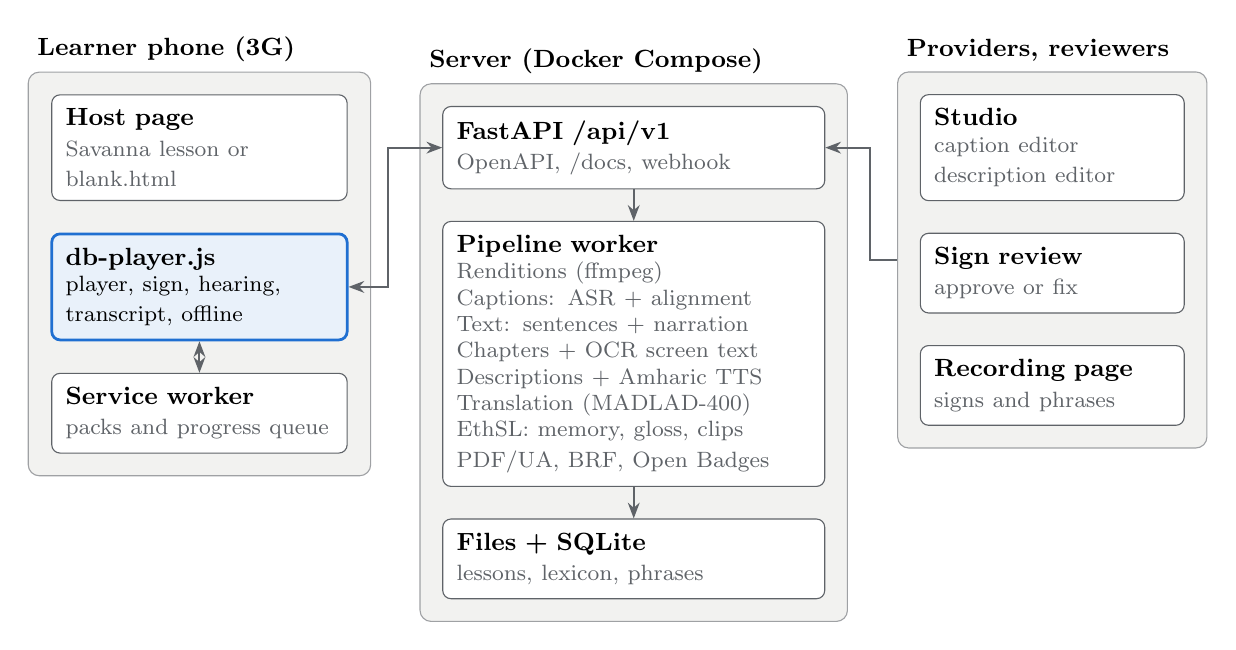
\begin{tikzpicture}[
  font=\small,
  box/.style={draw=quiet, rounded corners=3pt, align=left, text width=3.4cm, inner sep=5pt, fill=white},
  key/.style={box, draw=accent, fill=accent!10, line width=1pt},
  cont/.style={draw=quiet!60, rounded corners=4pt, fill=tint, inner sep=8pt},
  arr/.style={{Stealth[length=2mm]}-{Stealth[length=2mm]}, quiet, line width=0.7pt},
  one/.style={-{Stealth[length=2mm]}, quiet, line width=0.7pt}]

% phone column
\node[box] (host) {\textbf{Host page}\\{\color{quiet}\footnotesize Savanna lesson or blank.html}};
\node[key, below=4mm of host] (mod) {\textbf{db-player.js}\\{\footnotesize player, sign, hearing,\\ transcript, offline}};
\node[box, below=4mm of mod] (sw) {\textbf{Service worker}\\{\color{quiet}\footnotesize packs and progress queue}};

% server column
\node[box, right=1.2cm of host, text width=4.5cm] (api) {\textbf{FastAPI /api/v1}\\{\color{quiet}\footnotesize OpenAPI, /docs, webhook}};
\node[box, below=4mm of api, text width=4.5cm] (work) {\textbf{Pipeline worker}\\{\color{quiet}\footnotesize Renditions (ffmpeg)\\ Captions: ASR + alignment\\ Text: sentences + narration\\ Chapters + OCR screen text\\ Descriptions + Amharic TTS\\ Translation (MADLAD-400)\\ EthSL: memory, gloss, clips\\ PDF/UA, BRF, Open Badges}};
\node[box, below=4mm of work, text width=4.5cm] (store) {\textbf{Files + SQLite}\\{\color{quiet}\footnotesize lessons, lexicon, phrases}};

% people column
\node[box, right=1.2cm of api, text width=3.0cm] (studio) {\textbf{Studio}\\{\color{quiet}\footnotesize caption editor\\ description editor}};
\node[box, below=4mm of studio, text width=3.0cm] (review) {\textbf{Sign review}\\{\color{quiet}\footnotesize approve or fix}};
\node[box, below=4mm of review, text width=3.0cm] (rec) {\textbf{Recording page}\\{\color{quiet}\footnotesize signs and phrases}};

\begin{scope}[on background layer]
\node[cont, fit=(host)(mod)(sw), label={[font=\small\bfseries, anchor=south west]north west:Learner phone (3G)}] (c1) {};
\node[cont, fit=(api)(work)(store), label={[font=\small\bfseries, anchor=south west]north west:Server (Docker Compose)}] (c2) {};
\node[cont, fit=(studio)(review)(rec), label={[font=\small\bfseries, anchor=south west]north west:Providers, reviewers}] (c3) {};
\end{scope}

\draw[arr] (mod.east) -- ++(0.5,0) |- (api.west);
\draw[arr] (mod.south) -- (sw.north);
\draw[one] (api.south) -- (work.north);
\draw[one] (work.south) -- (store.north);
\draw[one] (c3.west) -- ++(-0.35,0) |- (api.east);
\end{tikzpicture}
\end{center}

The player talks to the API over HTTPS for tracks and media; providers and reviewers use the Studio pages, and the worker writes every output to files and SQLite. Phone tests run over an HTTPS tunnel; every AI step has a no-AI fallback.

\subsection{Stack}
\begin{xltabular}{\textwidth}{@{}>{\raggedright\arraybackslash}p{2.6cm} X >{\raggedright\arraybackslash}p{4cm}@{}}
\toprule
\textbf{Layer} & \textbf{Choice} & \textbf{Why} \\
\midrule
\endhead
Module & Vanilla web components, shadow DOM, about 60 KB & Works in any host, light on 3G \\
Captions & faster-whisper (English), Omnilingual ASR (Amharic), human editor & Open, CPU-capable \\
Alignment & torchaudio forced alignment & Word-level timing for Amharic \\
Translation & MADLAD-400 & Apache 2.0, covers Amharic \\
OCR & Tesseract \code{eng+amh} & Free, Ethiopic support \\
Media & ffmpeg & Renditions, slides, sign clips, crossfades \\
Amharic voice & Open TTS model behind one function & Swappable; licence checked \\
EthSL & HornMorpho, sentence embeddings, pluggable LLM, rule engine, ffmpeg; MediaPipe (stretch) & Layered pipeline in section~\ref{sec:ethsl} \\
Documents & WeasyPrint (PDF/UA), liblouis (BRF) & Open, tagged output \\
Certificates & Open Badges 3.0 signed JSON & Level 3 standard \\
API & FastAPI & OpenAPI and Swagger UI built in \\
Storage & SQLite + files & No database server to install \\
Tests & Playwright + axe-core, pytest & Gate check as a script \\
Deploy & Docker Compose: nginx (savanna, module, demo) + api + worker & One command \\
\bottomrule
\end{xltabular}

\subsection{Repository layout}
\begin{verbatim}
your-repo/
|-- README.md  docker-compose.yml  .env.example  CONFORMANCE.md  openapi.yaml
|-- module/   db-player.js, db-job-card.js, sw.js, i18n/en.json, i18n/am.json
|-- api/      FastAPI app, worker, pipeline steps, studio pages
|-- demo/     blank.html, data/ (lesson clip, VTT files, jobs.json, lexicon)
`-- savanna/  starter unchanged + our script tag; pages/jobs.html
\end{verbatim}

% ---------------------------------------------------------------- 12
\section{Acceptance tests and submission checklist}

Each user group has a short test that the co-designer runs unaided on their own phone; the submission is the four items the guide names.

\subsection{Acceptance tests}
\begin{xltabular}{\textwidth}{@{}l >{\raggedright\arraybackslash}p{2.6cm} X@{}}
\toprule
\textbf{ID} & \textbf{User} & \textbf{Test (unaided, own device)} \\
\midrule
\endhead
AT-01 & All & Install on \code{demo/blank.html} and the Savanna lesson page with one script tag; both look right \\
AT-02 & All & Main task with keyboard only, NVDA, TalkBack, 200\% zoom, sound off \\
AT-03 & Deaf & Turn on Sign, watch the signer large, lesson waits for the signer, tap ``variable'' and see its sign \\
AT-04 & Deaf & Move and resize the sign window by touch, by keyboard, and with the position buttons \\
AT-05 & Deaf & Rate 10 held-out auto-signed lines: understood / partly / not; target 90\% understood among published lines \\
AT-06 & Blind & Jump to Chapter 2 by heading, open ``What's on screen'' and read the code line by line \\
AT-07 & Blind & Hear a description pause and resume the video; change description volume \\
AT-08 & Hard of hearing & Turn on Clear voice on a cheap speaker; press ``Say that again'' twice; switch to mono \\
AT-09 & Hard of hearing & Move captions below the video and make them larger; settings remembered after reload \\
AT-10 & Slow connection & With Data Saver on, the light lesson is recommended with its size \\
AT-11 & Slow connection & Interrupt a download; it resumes; finish the lesson in aeroplane mode \\
AT-12 & Slow connection & Share the lesson file via Telegram and open it on another phone with no internet \\
AT-13 & Career & Job card read by TalkBack at 200\% zoom; ``Listen to summary'' plays; Ethiopian date shown \\
AT-14 & Career & Open the certificate verify link; it says ``valid''; a tampered copy says ``not valid'' \\
AT-15 & Judge & \code{docker compose up} on a clean laptop and install from the README within one hour \\
AT-16 & Text lesson & On the Savanna concept page, turn on Sign and Listen; sentences highlight while signed and narrated \\
\bottomrule
\end{xltabular}

\subsection{Submission (Sunday 16:30)}
\begin{itemize}[label=$\square$]
  \item Code under ALX's open licence, every library listed
  \item \code{README.md} in the guide's outline, including measured Slow 3G load time and size, caption and EthSL quality, cost for 3,000 learners, finished and not finished
  \item \code{docker-compose.yml} with \code{.env.example}
  \item \code{CONFORMANCE.md} (WCAG 2.2 AA)
  \item \code{openapi.yaml} and Swagger UI at \code{/docs}
  \item Repo layout: \code{module/}, \code{api/}, \code{demo/blank.html}, \code{demo/data/}, \code{savanna/} unchanged plus our script tag
\end{itemize}

\subsection{Checkpoints from the guide}
\begin{xltabular}{\textwidth}{@{}l X@{}}
\toprule
\textbf{When} & \textbf{What must be true} \\
\midrule
\endhead
Sat 17:00 & Main task works end to end, roughly; co-designer has tried it on their phone over HTTPS \\
Sun 12:00 & Must-haves added and tested; axe clean; Amharic complete \\
Sun 14:00 & Stop adding features; Level 2 documented; README and conformance written; compose tested on another laptop \\
Sun 15:30 & Co-designer final test; fix only blockers \\
Sun 16:30 & Submit \\
\bottomrule
\end{xltabular}

% ---------------------------------------------------------------- 13
\section{Risks and open questions}

The biggest risk is building too much: the main task must pass the gate before any extra is added.

\subsection{Risks and fallbacks}
\begin{xltabular}{\textwidth}{@{}>{\raggedright\arraybackslash}p{5.6cm} X@{}}
\toprule
\textbf{Risk} & \textbf{Fallback} \\
\midrule
\endhead
Feature load breaks the gate & Build the main task first; extras only after AT-02 passes \\
Automatic EthSL quality below target & Confidence gate publishes only high-confidence lines; low ones show captions plus glossary signs; report measured numbers honestly \\
Too few signs recorded on day 1 & Prioritise whole lesson phrases, then the demo lesson's vocabulary, then fingerspelling \\
Amharic ASR poor on our clip & Human-corrected Amharic captions for the demo; state measured quality \\
Web Audio silent on cross-origin video & Serve video from the same origin or with CORS headers \\
TalkBack behaves differently from NVDA & Test on the co-designer's phone every few hours from day 1 \\
Android blocks opening a shared HTML file & Share a link to the in-app download instead \\
Translation and TTS models slow on CPU & Pre-generate the demo lesson's outputs; say so \\
Service worker and camera fail on plain HTTP & Use a \code{cloudflared} tunnel for every phone test \\
Licence of a model unclear & Keep it behind the swappable interface; use rules or no-AI mode \\
\bottomrule
\end{xltabular}

\subsection{Open questions (to answer with mentors and co-designers)}
\begin{itemize}[label=$\square$]
  \item Which open licence did ALX name at kick-off?
  \item Do agreed EthSL signs exist for core tech terms (variable, function, loop, API)? Who confirms them?
  \item Which 10 grammar rules do the interpreters use for lesson sentences?
  \item Consent wording for recorded signers, and how they are credited.
  \item Which Amharic TTS model has a licence ALX accepts?
  \item Rough monthly cost for 3,000 learners (storage, CPU for the pipeline, optional AI calls).
  \item Guide question: how small can a useful offline lesson be? Proposed answer: Text pack, about 50 KB.
  \item Guide question: what happens when a lesson has no sign video yet? Proposed answer: FR-DEAF-08 plus the automatic pipeline.
\end{itemize}

\end{document}
